% Should be ~50% of the whole thesis
\iffalse
\begin{itemize}
	\item Don’t make the reader do all the work
	\item Have a hypothesis, test them, state result clearly
	\item Two lists are not a comparison
	\item Be the first to criticize your own work
\end{itemize}
\fi
\
\section{Hardware results}
The configuration and setup between the load cell and ADC took some time to get right, mostly due a faulty load cell being used during the first half of the project. It was also assumed that the color of the wires was standardized between load cells, so the correct wiring in figure \ref{fig:load_cell_hx711} was not implemented right away. Even though no calibrations were made to the load cell during this paper, an increase in the voltage provided to the load cell did correlate to an increased stability in the values produced. 

The second big challenge involving the hardware came from powering the project in a sufficient manner. The first power setup as seen in figure \ref{fig:wiring_comp}, was a simple and naive approach that lacked enough voltage to efficiently power the components. The benefit of this setup was a simple wiring schema where each component powered the next in line. The drawback was that the FiPy could only supply the ADC with 3V, which in turn affected the ADC's ability to read data from the load cell. During testing, the output rate of the raw data would be infrequent and erratic, sometimes taking several seconds to produce a single value. The values themselves did not correspond to increases and decreases in force being applied to the load cell, and would seemingly spike and crash at random. These problems were largely in part due to the insufficient voltage being supplied to the ADC and load cell as later setups would reveal.

% Second wiring setup
The second wiring setup was the one seen in figure \ref{fig:wiring_outlet}, and resulted in an electrical interference throughout the system, because of two different grounds being present in the circuit. This electrical interference rendered the output of the system nonsensical at time, though output rate of the data values had improved to a bit more stable rhythm than previously, and the raw data values were a bit more responsive to the force applied to the load cell..

% Third wiring setup
The third and final power setup for the project involved the Otii battery toolbox, as seen in figure \ref{fig:wiring_otii}. This setup, though a bit too advanced for a device intended to be small and simple, did produce a functioning connection between the load cell and the microcontroller. When force was applied to the load cell, the data values responded accordingly with an increase or decrease in value, and no irregularities in form of disconnects or spikes were seen in the tests. Due to time constraints and hardware availability, the setup could not be used for real network transmissions of the load cell data.

\section{Software results}

\subsection{reader.py}
The \lstinline{reader.py} file contains the \lstinline{Reader} class, which is responsible for processing the data polled from the load cell and passing it on to being transmitted. To instantiate a functional \lstinline{reader} object, it needs to be passed a poller function as well as a transmitter function. The purpose of having these functions passed to the instance of the class instead of being hardcoded into the class is to follow the separation of concern design principle.\cite{sep-concern} The type signatures for the two functions are show below. The poller function should accept no argument and is expected to return the current data value produced by the load cell when called. The transmitter function can accept a argument of any type, and should not return any value.
\begin{Code}
	def poller_function() -> value: int
	def transmitter_function(value: Any): -> None
\end{Code}


The main method of the \lstinline{reader} instance is the \lstinline{run()} method. When called, the \lstinline{run()} method performs a cycle consisting of data polling, a check for false values, adjustment of the polling rate as well as a possible transmission. 

\subsubsection{Error Check}
The polled data value is subsequently checked for validity in the form of out-of-bounds values or extreme delta changes. A separate class called \lstinline{Error_tracker} monitors the interval and frequency of these occurrences, and the purpose of the class is to raise an exception when the error rate is deemed too high, and some form of remedial action needs to be taken. The internal workings of the \lstinline{Error_tracker} will be explained in a separate section.

%TODO
\subsubsection{Disconnect Check}


\subsubsection{Adjustment of polling rate}
If the value is deemed valid, it is added to a First-in, First-out (FIFO) buffer of the most recent values. The contents of the buffer are then summed into a total delta value, which is used to adjust the polling rate. If the total delta surpasses a pre-defined threshold, the polling rate is increased, whereas if it is lower it might be maintained or decreased. The total delta value is the the delta values between two points added to the delta of the next two points, as follows:

$$\sum_{n=0}^{10} x_n - x_{n+1}$$


\subsection{error\_tracker.py}
The purpose of the Error\_tracker class is to keep track of the error occurrence and frequency. The intended usage is to instantiate an instance of the class, and call the \lstinline{error_occurred()} method when an invalid read has occurred. This method increases an internal counter, which will then raise an exception if it passes a pre-defined threshold.

\subsubsection{The Grace Period}
When invalid reads occur due to some temporary circumstance, it might not be beneficial to count all errors within a given timeframe towards raising an exception. It is not useful sending an alert when short periods of errors occur (given that very high uptime is not of importance), since this might risk producing a multitude of needless error messages. Instead, it is at the long-lasting periods of polling errors an exception should be raised. To account for short bursts of error, a constant called \lstinline{GRACE_PERIOD} is used. This constant measures the time window (in seconds) after the \lstinline{error_occurred()} method has been called, during which sequential calls  will not count toward the exception threshold.

\subsubsection{The Cooldown Period}
If errors rack up towards an exception over a longer period of time, it would lose meaning in regards to the status of the device in the short term, and would only be an indicator of long-term performance. To avoid this, the internal error counter needs to be reset or decreased periodically. To achieve this, a constant similar to the \lstinline{GRACE_PERIOD} is used, called the \lstinline{COOLDOWN} constant. This constant indicates the time window (in seconds) after the grace period, where if no calls are made to the \lstinline{error_occurred()} method, the internal error counter is decreased by one. However, if a call to the \lstinline{error_occurred()} method is made during the cooldown period, the internal error counter increases, and a new grace period starts. This way of self-regulation ensures that only a long-lasting and consistent frequency of errors raise an exception.


\subsection{Data Transmissions}
Data transmission tests were done separately from the load cell using fictional data. Pycom, the parent company behind the microcontroller used in this project also operate a cloud-based device management platform. \cite{pybytes-website} Via the pybytes platform, configuration of the network settings of the device can be managed via a firmware updater. 
In figure \ref{fig:wifi_longterm} and figure \ref{fig:wifi_raw_values} we can see data being transmitted via Wifi on a home network. The data is then displayed via graphs on the pybytes platform.

\begin{figure}[H]
\centering
	\begin{subfigure}[b]{0.4\textwidth}
    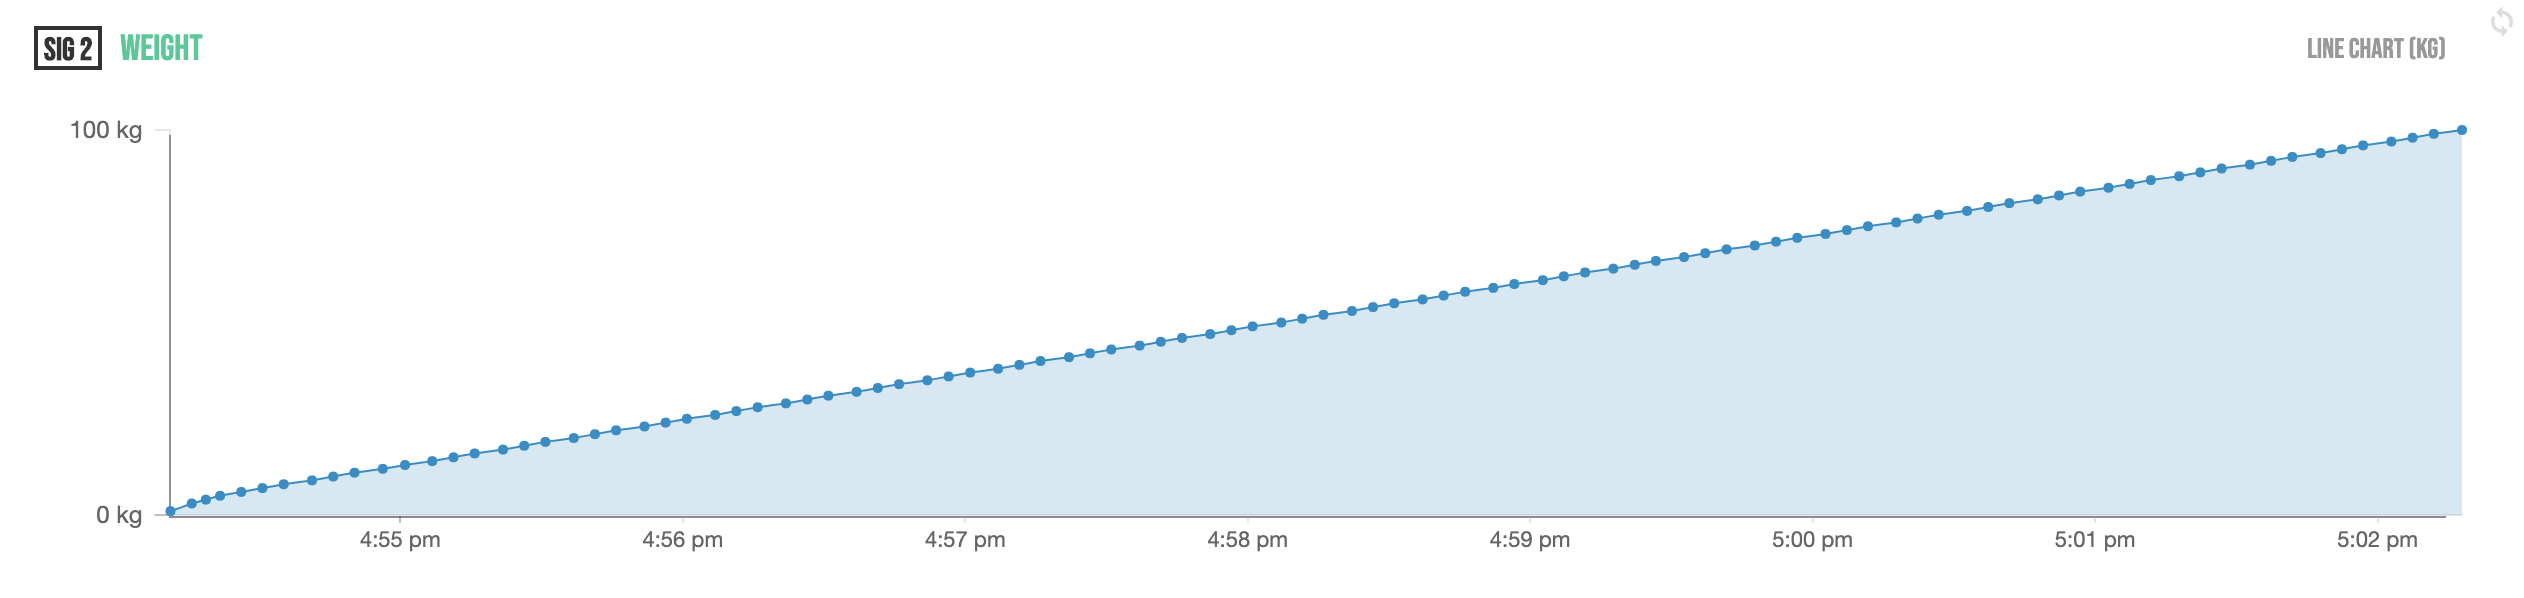
\includegraphics[width=\textwidth]{wifi_longterm.png}
    \caption{Data transmitted via Wifi}
    \label{fig:wifi_longterm}
	\end{subfigure}
	%
	\begin{subfigure}[b]{0.4\textwidth}
    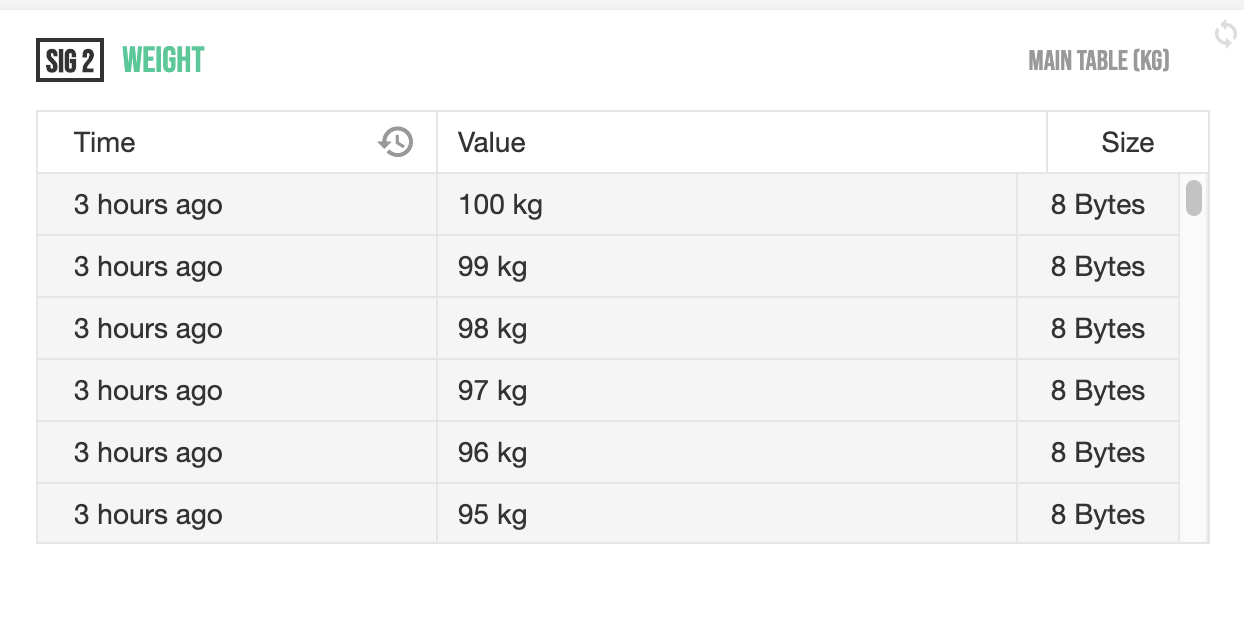
\includegraphics[width=\textwidth]{wifi_raw_values.png}
    \caption{Values transmitted via Wifi}
    \label{fig:wifi_raw_values}
	\end{subfigure}
\end{figure}

Due to time limitations in the project, no actual tests of the transmission of the data via NB-IoT were performed.
%TODO: Write more here

\section{Discussion}
%Interpretations: what do the results mean?
Despite hardships and complications when implementing the hardware, the results suggest that building and programming an NB-IoT enabled device connected to a load cell is possible with fairly simple consumer available hardware devices. It is a reasonable assumption that the hardware hindrances encountered in this paper can be bypassed with adequate planning and experience in assembling electric hardware.

%Implications: why do the results matter?
These results show a small starting point of implementing a IoT device using a load cell as its sensor. With the rise of 5G and IoT platform services there exists a real commercial interest to enable more and more actors to innovate and create products for consumers and companies alike. This project can serve as a starting point for what design and requirement considerations regarding hardware and software that need to be considered when planning and designing such a device.

\subsection{Limitations}
%Limitations: what can’t the results tell us?
%% Long term functionality
The most glaring issue with the way the hardware and software were tested during this project pertains to the time duration. When testing the connection between the load cell and microcontroller, as well as transmitting the data from the microcontroller, the tests were short compared to the intended %%TODO
%% Mass production
This project was done on a small scale, and extensive research in multiple different areas need to be conducted to even get a IoT enabled scale close to being produced for functional use, commercial or private.
%% Variance for customer
Furthermore, these results cannot account for whether the software implementation was close to emulating the desired behavior of a device from a practical standpoint, since no potential end-users were involved in the requirement specification.
%% Real life environments
Since the testing was only done indoors in a clean and controlled environment, unknown variables present in the real world could very well produce a multitude of challenges that change the way that the device works. Another interesting angle is how different locations would interact with the connection to the cellular network the NB-IoT SIM-card relies on for communication. The NB-IoT technology makes huge promises, but at the end of the day it is up to the local telecom company to fulfill the underlying conditions that make those claims possible, which would be Telia in our case.
% Duration of transmission, failure handling

% Different operators
Expanding on this, since the NB-IoT technology is fairly new in a lot of countries, there is bound to be extremely different implementation experiences from region to region depending on the network provider. In fact, NB-IoT devices could be rendered obsolete in entire regions depending on the network provider.
